\chapter{Related Work}
\label{cha:relatedwork}

\section{Approaches to stop detection for localization services}
\label{cha:introduction_appr_stopdet}

\subsection{Stop Detection analyzing repetitive appearance at location}

\subsection{Stop Detection based on continuous localization}

\subsection{Stop Detection based on mobility index}
\label{cha:introduction_mob_index_sect}

In the paper \cite{MobilityIndexGIS}, movement of mobile devices between cells (handovers) is considered. To detect the periods of slow movements of stops at the specific location, parameter called Mobility Index is considered. 
\begin{figure}[!ht]
	\centering
	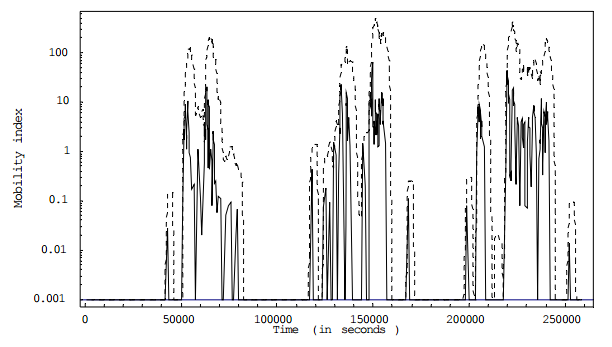
\includegraphics[width=0.5\textwidth]{images/intro_mobility_index.png}\\
	\caption{Mobility Index. Source: \cite{MobilityIndexGIS}}
	\label{fig:introduction_mob_index}
\end{figure}
\\
In a populated area, with many GSM cells, the mobile
terminal can change from one cell to another within
seconds or after several minutes. Given a set of consecutive records, the mobility of a user can be estimated by calculating the Mobility Index over a pre-defined time period (sliding window). 
\\\\
The Mobility Index is defined as the sum of the "distances" between each record and the previous ones, where the "distance" is the inverse of the time spent on each cell. If the value of MI is below certain threshold, it is assumed that the object stopped or moved slowly. 
\\\\
In the publication, sliding window of 10 minutes and a mobility index threshold value of 6 has been used for certain area. The obtained results were in agreement with actual movements during more than 90\% of the time. 
\\\\
High mobility index tells that user have been moving from checkpoint to checkpoint within very small time distance. Rapid drop in mobility index represents very long duration at the last point, and slight decrease in mobility index means that user changed position, but within longer duration.